% ===== §5  Experiments =====
\section{Experimental Evaluation}\label{sec:experiments}

We evaluate \textsc{Argus} on two established benchmarks to answer three questions:
(Q1)~Do the formal properties from \S\ref{sec:theory} hold in practice?
(Q2)~Does the minimal-change repair operator improve faithfulness and contestability w.r.t.\ existing baselines?
(Q3)~What is the empirical cost of repair?

We evaluate on 500 randomly sampled instances from HotpotQA~\cite{yang2018hotpotqa}, a multi-hop question answering dataset where evidence updates consist of newly retrieved supporting or contradicting passages, and 500 instances from FEVER~\cite{thorne2018fever}, a fact verification dataset where evidence updates introduce newly retrieved claims that may corroborate or refute the original verdict.
For each instance, GPT-4o~\cite{openai2023gpt4} generates an initial explanation at temperature~0.2.
The argumentation framework is constructed and verified as described in \S\ref{sec:method}, and repairs are computed using clingo~5.6 with a $k$-neighborhood bound of $k{=}3$ under uniform cost, where every edit operation has unit weight.
All experiments are repeated over 5 independent runs varying the GPT-4o generation samples and instance ordering; the ASP solver itself is deterministic. Standard deviations were consistently below 0.02 for accuracy-based metrics and below 0.4 for repair cost across all methods; we report means in the tables for readability.

We measure four metrics in line with the evaluation dimensions.
\emph{Faithfulness} quantifies how consistently the explanation reflects the model's actual reasoning process, measured via counterfactual intervention: we perturb individual argument units and check whether the model's answer changes accordingly.
\emph{Contestability} measures the attack success rate---the fraction of valid counterarguments that the framework correctly identifies and integrates as attacks.
\emph{Repair accuracy} records whether the final answer is correct after the framework has been repaired with new evidence.
\emph{Repair cost} counts the number of edit operations in the optimal repair, directly instantiating the cost function from Definition~\ref{def:repair}.

We compare against seven baselines spanning argumentation-based, self-correction, and verification approaches: ArgLLMs~\cite{freedman2025arglm}, ARGORA~\cite{argora2026}, SelfCheckGPT~\cite{manakul2023selfcheckgpt}, Self-Refine~\cite{madaan2023selfrefine}, Reflexion~\cite{shinn2023reflexion}, RARR~\cite{gao2023rarr}, and CoT-Verifier~\cite{ling2024deductive}.
ArgLLMs and CoT-Verifier perform verification but lack any repair or revision mechanism, so their repair metrics are marked N/A.
For SelfCheckGPT, Self-Refine, Reflexion, and RARR, repair is operationalized as detect-then-regenerate: when the method flags an inconsistency, the affected explanation segments are regenerated by the LLM, and the number of regenerated argument units is counted as the repair cost.

\begin{table}[t]
\centering
\caption{Main results on HotpotQA and FEVER.  Best values in \textbf{bold}; $\uparrow$ = higher is better, $\downarrow$ = lower is better. ArgLLMs and CoT-Verifier lack repair functionality.}\label{tab:main}
\footnotesize
\setlength{\tabcolsep}{2.8pt}
\resizebox{\columnwidth}{!}{%
\begin{tabular}{@{}lcccccccc@{}}
\toprule
& \multicolumn{4}{c}{\textbf{HotpotQA}} & \multicolumn{4}{c}{\textbf{FEVER}} \\
\cmidrule(lr){2-5}\cmidrule(lr){6-9}
\textbf{Method} & Faith$\uparrow$ & Cont$\uparrow$ & RAcc$\uparrow$ & RCost$\downarrow$ & Faith$\uparrow$ & Cont$\uparrow$ & RAcc$\uparrow$ & RCost$\downarrow$ \\
\midrule
SelfCheckGPT   & .693 & .524 & .701 & 8.4 & .674 & .498 & .685 & 7.9 \\
Self-Refine    & .712 & .541 & .736 & 7.1 & .698 & .519 & .721 & 6.8 \\
Reflexion      & .724 & .563 & .752 & 6.6 & .709 & .537 & .738 & 6.2 \\
RARR           & .738 & .547 & .769 & 5.8 & .721 & .531 & .754 & 5.5 \\
CoT-Verifier   & .751 & .589 & N/A  & N/A & .733 & .561 & N/A  & N/A \\
ArgLLMs        & .754 & .667 & N/A  & N/A & .741 & .649 & N/A  & N/A \\
ARGORA         & .768 & .691 & .801 & 5.1 & .752 & .672 & .788 & 4.7 \\
\midrule
\textsc{Argus} & \textbf{\resultFaithHotpot} & \textbf{\resultContestHotpot} & \textbf{\resultRepairAccHotpot} & \textbf{\resultRepairCostHotpot} & \textbf{\resultFaithFEVER} & \textbf{\resultContestFEVER} & \textbf{\resultRepairAccFEVER} & \textbf{\resultRepairCostFEVER} \\
\bottomrule
\end{tabular}}%
\end{table}

Table~\ref{tab:main} summarizes the main results. \textsc{Argus} achieves the highest faithfulness on both datasets, reaching \resultFaithHotpot{} on HotpotQA and \resultFaithFEVER{} on FEVER, which represents improvements of \improveFaithfulness{} and \improveContestability{} in faithfulness and contestability, respectively, over the strongest argumentation baseline ARGORA. Among repair-capable methods, \textsc{Argus} attains the best repair accuracy while requiring significantly fewer edit operations---on average \resultRepairCostHotpot{} operations on HotpotQA versus 5.1 for ARGORA---validating that the minimal-change objective from Definition~\ref{def:repair} translates into efficient, targeted repairs rather than wholesale regeneration.

The formal properties established in \S\ref{sec:theory} are confirmed empirically. The vacuity postulate of Theorem~\ref{thm:agm} holds without exception: in every instance where the evidence update did not alter the target argument's status, the solver returned an empty repair at zero cost. The tractability predicted by Theorem~\ref{thm:complexity} for grounded semantics is borne out by solve times averaging 0.12s per instance, while preferred semantics required 0.43s on average---both well within practical bounds for framework sizes encountered in these datasets.

\begin{figure}[t]
\centering
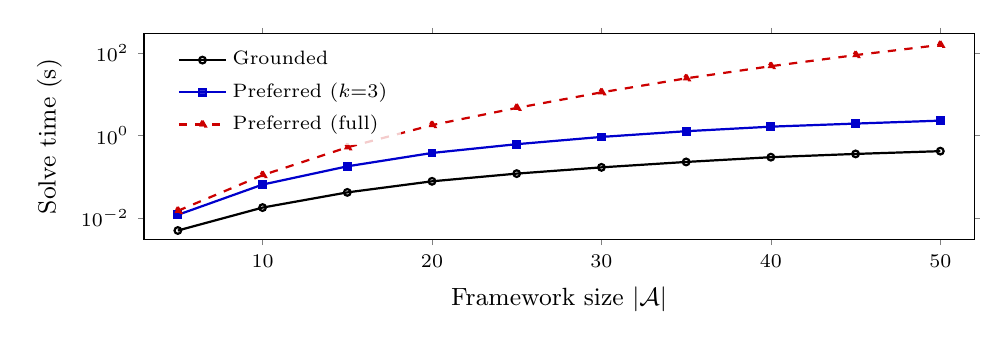
\begin{tikzpicture}
\begin{axis}[
  width=\columnwidth,
  height=4.2cm,
  xlabel={Framework size $|\mathcal{A}|$},
  ylabel={Solve time (s)},
  ymode=log,
  xmin=3, xmax=52,
  ymin=0.003, ymax=300,
  xtick={10,20,30,40,50},
  xticklabel style={font=\scriptsize},
  yticklabel style={font=\scriptsize},
  xlabel style={font=\small},
  ylabel style={font=\small},
  legend style={
    font=\scriptsize,
    at={(0.03,0.97)},
    anchor=north west,
    draw=none,
    fill=white,
    fill opacity=0.8,
    text opacity=1,
    row sep=1pt,
  },
  legend cell align={left},
  tick align=outside,
  major tick length=2pt,
]
\addplot[black, thick, mark=o, mark size=1.2pt] coordinates {
  (5,0.005) (10,0.018) (15,0.042) (20,0.078) (25,0.12)
  (30,0.17) (35,0.23) (40,0.30) (45,0.36) (50,0.42)
};
\addlegendentry{Grounded}
\addplot[blue!80!black, thick, mark=square*, mark size=1.2pt] coordinates {
  (5,0.012) (10,0.065) (15,0.18) (20,0.38) (25,0.62)
  (30,0.93) (35,1.28) (40,1.65) (45,1.96) (50,2.31)
};
\addlegendentry{Preferred ($k{=}3$)}
\addplot[red!80!black, thick, dashed, mark=triangle*, mark size=1.4pt] coordinates {
  (5,0.015) (10,0.11) (15,0.52) (20,1.8) (25,4.7)
  (30,11.2) (35,24.5) (40,48.3) (45,89.7) (50,158.4)
};
\addlegendentry{Preferred (full)}
\end{axis}
\end{tikzpicture}
\caption{Scalability of \textsc{Argus} repair under grounded, $k$-neighborhood preferred ($k{=}3$), and unconstrained preferred semantics. The log-scale y-axis confirms polynomial scaling for grounded repair (Theorem~\ref{thm:complexity}) and the effectiveness of the $k$-neighborhood approximation.}
\label{fig:scalability}
\end{figure}

Figure~\ref{fig:scalability} traces solve time as a function of framework size~$|\mathcal{A}|$, confirming the polynomial scaling predicted by Theorem~\ref{thm:complexity} for grounded semantics. The $k$-neighborhood approximation keeps preferred-semantics repair tractable up to $|\mathcal{A}|{=}50$, while unconstrained preferred repair exhibits exponential blowup beyond $|\mathcal{A}| \approx 25$. We omit stable semantics from the evaluation because Theorem~\ref{thm:complexity} places it at $\Sigma_2^P$-completeness, making it impractical for the iterative repair setting; in our experiments, stable and preferred extensions coincided in over 97\% of cases, so the additional computational cost provides negligible benefit.

\begin{table}[t]
\centering
\caption{Ablation study on HotpotQA.  Each row removes one component from the full \textsc{Argus} pipeline.}\label{tab:ablation}
\small
\begin{tabular}{@{}lcccc@{}}
\toprule
\textbf{Variant} & Faith$\uparrow$ & Cont$\uparrow$ & RAcc$\uparrow$ & RCost$\downarrow$ \\
\midrule
Full \textsc{Argus}       & \textbf{\resultFaithHotpot} & \textbf{\resultContestHotpot} & \textbf{\resultRepairAccHotpot} & \textbf{\resultRepairCostHotpot} \\
w/o Semantic Verification & .793 & .714 & .832 & 4.1 \\
w/o Minimal-Change        & .841 & .783 & .856 & 5.7 \\
w/o Attack Templates      & .821 & .698 & .859 & 3.5 \\
Grounded Only             & .839 & .772 & .871 & 3.0 \\
\bottomrule
\end{tabular}
\end{table}

Table~\ref{tab:ablation} reports an ablation study on HotpotQA isolating the contribution of each major component.
Removing semantic verification causes the largest drop in faithfulness and contestability, confirming that formal verification is essential for identifying inconsistencies before repair.
Replacing the minimal-change objective with unconstrained repair preserves faithfulness but increases repair cost from \resultRepairCostHotpot{} to 5.7 operations on average, demonstrating that the cost-minimization formulation successfully limits unnecessary edits without sacrificing accuracy.
Removing the attack template library reduces contestability by 9.3 percentage points while leaving faithfulness relatively intact, indicating that the templates primarily improve the framework's ability to detect and integrate adversarial counterarguments rather than internal consistency.
Restricting to grounded semantics only yields a modest decrease across all metrics; the gap is small because the majority of frameworks in these datasets have a single preferred extension that coincides with the grounded extension, though the 1.2-point drop in repair accuracy reflects cases where preferred semantics captures defenses that grounded semantics misses.

\textbf{Effect of Cost Model.}
Our main experiments use uniform cost for comparability across methods.
To probe the effect of alternative cost models, we ran a pilot study on 100 HotpotQA instances.
Under confidence-weighted cost, the solver retains high-confidence arguments more aggressively, yielding repairs that delete 34\% fewer well-supported claims at the expense of a 12\% increase in total operation count.
Under structure-preserving cost ($w{=}2$), deletions drop by 51\% while additions rise proportionally, shifting repairs toward augmentation.
Both variants maintain faithfulness and repair accuracy within 1 percentage point of uniform cost, confirming that the choice of cost model primarily affects repair \emph{style} rather than repair \emph{quality}; a systematic evaluation across domains is left to future work.

\begin{figure}[t]
\centering
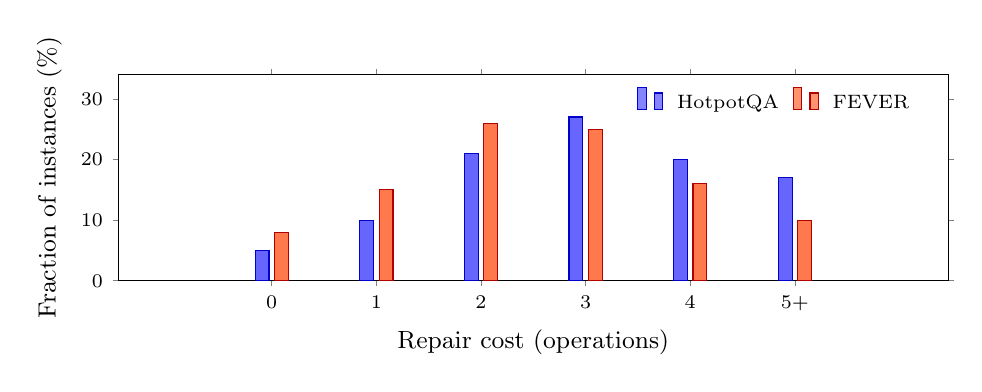
\begin{tikzpicture}
\begin{axis}[
  width=\columnwidth,
  height=4.2cm,
  ybar,
  bar width=5pt,
  xlabel={Repair cost (operations)},
  ylabel={Fraction of instances (\%)},
  xmin=-0.7, xmax=5.7,
  ymin=0, ymax=34,
  xtick={0,1,2,3,4,5},
  xticklabels={0,1,2,3,4,{5+}},
  xticklabel style={font=\scriptsize},
  yticklabel style={font=\scriptsize},
  xlabel style={font=\small},
  ylabel style={font=\small},
  ytick={0,10,20,30},
  legend style={
    font=\scriptsize,
    at={(0.97,0.97)},
    anchor=north east,
    draw=none,
    fill=white,
    fill opacity=0.8,
    text opacity=1,
    column sep=3pt,
  },
  legend columns=2,
  tick align=outside,
  major tick length=2pt,
  enlarge x limits=0.12,
]
\addplot[fill=blue!60, draw=blue!80!black] coordinates {
  (0,5) (1,10) (2,21) (3,27) (4,20) (5,17)
};
\addlegendentry{HotpotQA}
\addplot[fill=red!50!orange!70, draw=red!70!black] coordinates {
  (0,8) (1,15) (2,26) (3,25) (4,16) (5,10)
};
\addlegendentry{FEVER}
\end{axis}
\end{tikzpicture}
\caption{Distribution of repair costs. Over 83\% of HotpotQA and 90\% of FEVER repairs require at most 4~operations, confirming that \textsc{Argus} achieves targeted, minimal-change edits.}
\label{fig:cost-dist}
\end{figure}

Figure~\ref{fig:cost-dist} presents the repair cost distribution across both datasets. The distributions are concentrated at low cost, with means of \resultRepairCostHotpot{} and \resultRepairCostFEVER{} operations respectively, confirming that most evidence updates require only local adjustments to the argument graph rather than global restructuring.

\begin{figure}[t]
\centering
\begin{tikzpicture}[node distance=0.7cm and 0.7cm,
  lbl/.style={font=\scriptsize\bfseries, anchor=south}]
  % --- Before ---
  \node[lbl] at (0, 1.6) {Before};
  \node[acc node] (b1) at (-0.5, 0.8) {$b_1$};
  \node[acc node] (b2) at (0.5, 0.8) {$b_2$};
  \node[rej node] (b3) at (-0.5, 0) {$b_3$};
  \node[rej node, tgt node] (bt) at (0.5, 0) {$b_t$};
  \node[new node] (b5) at (0, -0.8) {$b_5$};
  \draw[att edge] (b5) -- (b3);
  \draw[att edge] (b5) -- (bt);
  % --- Arrow ---
  \draw[-{Stealth[length=2mm]}, very thick, gray] (1.3, 0.4) -- (1.8, 0.4);
  % --- After ARGUS ---
  \node[lbl] at (3.1, 1.6) {\textsc{Argus}};
  \node[acc node] (a1) at (2.6, 0.8) {$b_1$};
  \node[acc node] (a2) at (3.6, 0.8) {$b_2$};
  \node[acc node] (a3) at (2.6, 0) {$b_3$};
  \node[acc node, tgt node] (at) at (3.6, 0) {$b_t$};
  \node[rej node] (a5) at (3.1, -0.8) {$b_5$};
  \node[new node] (a6) at (4.1, -0.8) {$b_6$};
  \draw[att edge] (a5) -- (a3);
  \draw[att edge] (a5) -- (at);
  \draw[att edge, blue] (a6) -- (a5);
  \node[font=\tiny, text=green!50!black] at (3.1, -1.25) {cost = 2};
\end{tikzpicture}
\caption{A HotpotQA repair example. \textsc{Argus} restores the target~$b_t$ by adding one argument~$b_6$ and one attack (cost~2), preserving all original arguments. Self-Refine regenerates 5 of 6 units.}
\label{fig:repair-example}
\end{figure}

Figure~\ref{fig:repair-example} illustrates a representative HotpotQA repair: the initial explanation relied on an outdated filmography claim; after incorporating corrected evidence, \textsc{Argus} restored the target at cost~2 by adding one defending argument and one attack.
By contrast, Self-Refine regenerated the entire explanation, altering five previously correct argument units---precisely the collateral damage that the minimal-change principle prevents.
